

\chapter{Model predictive control for synchronous phase shifting of circadian oscillator populations}
\blfootnote{Major portions of this chapter appear as J.H.~Abel, A.~Chakrabarty, and F.J.~Doyle~III, ``Controlling time: nonlinear model predictive control for populations of circadian oscillators,'' in \textit{Emerging Applications of Control and System Theory}, R.~Tempo, S.~Yurkovich, P.~Misra Eds. New York, NY: Springer Publishing, 2018. ISBN: 978-3-319-67068-3. All theoretical and computational results were by J.H.\ Abel. Research approach was conceived in collaboration with and under the mentorship of F.J.\ Doyle III and A.\ Chakrabarty, with additional inspiration from the work of P.C.\ St.\ John.} 

\section{Introduction}
\label{sec:background}


High amplitude circadian oscillations are associated with good metabolic health \cite{Ramkisoensing2015}, commensurate with the broad integration of circadian regulation with metabolic function \cite{Panda2002, Bass2010}.
High amplitude oscillation within peripheral (i.e.\ non-neural) tissues of the body is achieved by high oscillatory amplitudes from the individual oscillators comprising the tissue, as well as a high degree of synchrony among the oscillator population \cite{Ukai2007,StJohn2014b,Gan2017}.
Since disruption to the circadian oscillator can take the form of either misaligned phase (as in the prior chapter) there is a need to develop therapies to mitigate the effects of disruption to the circadian clock, to rapidly re-align circadian phase with the environment following jet lag or shift work to avoid cognitive difficulty, and to promote high-amplitude circadian oscillation.
Since circadian rhythms are complex phenomena, phase, synchrony, and amplitude control of the clock may be better approached by control theory rather than an ad hoc approach to the delivery of drugs or light \cite{Bagheri2008, Serkh2014, Zhang2016}.

As mentioned in the previous chapter, control strategies devised for manipulation of mammalian circadian rhythms may analogously be applied to other oscillatory biological systems, provided they are well-described by limit-cycle oscillators.
Circadian oscillators in other species such as the KaiABC system in the cyanobacterium \textit{Synechococcus} \cite{Ishiura1998}, or the \textit{Period}-\textit{Timeless} oscillator in \textit{Drosophila} \cite{Glossop1999} have been modeled as limit-cycle oscillators for more than a decade.
More generally, genetic or phosphorylation-driven oscillators are a ubiquitous biological motif involved in the metabolic processes of numerous organisms from prokaryotes to mammals \cite{Huang2003, Goodwin1965}, and the development of strategies for manipulating both phase and synchrony of these systems is broadly desirable.
To-date, control of circadian rhythms has been 
A more detailed approach to control of circadian dynamics would integrate tissue or population-scale effects, pharmacokinetics and pharmacodynamics, and interactions between different oscillator populations.

Herein, we begin to approach this detailed formulation by presenting a MPC framework for manipulating phase and synchrony within populations of uncoupled biological oscillators using a pharmaceutical agent, and demonstrate the efficacy of such an approach by \textit{in silico} simulations of phase shifting in the mammalian clock.
We do so by describing the population of oscillators as a phase probability density function, as in \cite{StJohn2014b}, and using the parametric infinitesimal phase response curve (PRC) to calculate how the phase PDF evolves in response to control input.
By using a predictor that accounts explicitly for the variability in phase within a synchronized population, we are able to maintain synchrony of oscillators while performing a phase shift, unlike the single-oscillator case.


In this chapter, we present a framework for the control of a population of biological oscillators, motivated by the example of the mammalian circadian clock.
First, we use our previously-derived simplification of oscillator dynamics using the parametric phase response to a control input to reduce the dynamical model to a phase-only representation \cite{Abel2016b}: this is advantageous in reducing the dimensionality of the MPC problem, thereby curbing computational effort.
We then present a controller for the case for a single oscillator, designed using the principles of the previous chapter, and demonstrate its function \textit{in silico}.
Next we demonstrate that although this formulation may successfully control a single oscillator, applying this controller to manipulate mean phase of a population of oscillators may effect a desynchronization detrimental to biological function.
We then modify the MPC problem using a probability density function of population phase in conjunction with the simplified dynamics to exert simultaneous control over phase and synchrony within an oscillator population.
We demonstrate the \textit{in silico} efficacy of this approach in maintaining synchrony throughout a phase realignment.
Finally, we discuss limitations of this approach, and challenges to its implementation \textit{in vivo} and \textit{in vitro}.


\section{Control of a single circadian oscillator}
\label{sec:single}
A standard approximation in the control of the circadian oscillator is describing the targeted circadian system (i.e., the population of cells comprising clocks in brain or peripheral tissues such as the liver) as a single limit-cycle oscillator \cite{Slaby2007, Bagheri2007, Shaik2008, Bagheri2008, Serkh2014, Zhang2016, Abel2016b, Abel2017a}.
We begin our treatment of applying control to phase-shift the circadian oscillator by exploiting this approximation, as in our previous work \cite{Abel2016b, Abel2017a} as well as the prior chapter, to illustrate where it fails to capture population-scale phenomena.

\subsection*{Modeling the circadian oscillator}


As described in detail in Chapter 1, the mammalian circadian oscillator within an individual cell is comprised of interlocked transcriptional-translational feedback loops. 
The core negative feedback loop involves isoforms of the genes \textit{Period} (\textit{Per}) and \textit{Cryptochrome} (\textit{Cry}), which form PER-CRY heterodimers and enter the nucleus to bind to BMAL1-CLOCK E-box activators to repress their own transcription.
As these repressors are degraded, BMAL1-CLOCK dimers activate transcription of \textit{Per}s and \textit{Cry}s, resulting in a self-sustained oscillation.
Downstream of the circadian feedback loops, clock components regulate transcriptional architecture through D-box, E-box, and ROR-binding elements.
For an excellent review of the genetic components of the mammalian oscillator, see \cite{Takahashi2016}.

Numerous dynamical models of the circadian oscillator have been proposed.
In this work, as in the previous chapter, we selected the model from \cite{Hirota2012a, StJohn2014a}, as it was created to identify the effect of the small-molecule KL001 on the mammalian oscillator.
This model consists of 8 nonlinear coupled ODEs and 21 kinetic parameters, fully described in the supplement to \cite{StJohn2014a} and reproduced in Table~\ref{tab:stjohnmodel}.
Because KL001 was found to stabilize nuclear PER-CRY transcription factors, control is implemented in the model by modifying the ODEs describing the degradation of PER-CRY dimers as follows:
\begin{subeqnarray}
	\label{eq:cry1} 
   \frac{d\mathrm{C1P}}{dt} &=& v_{\mathrm{a,{CP}}} \mathrm{P} \cdot \mathrm{C1} - v_{\mathrm{d,{ CP}}} \mathrm{C1P} 
    - \frac{( v_\text{dCn-u(t)}) \mathrm{C1P} }{k_{\mathrm{deg,{Cn}}} +\mathrm{C1P}  + \mathrm{C2P} }\\
    \frac{d\mathrm{C2P }}{dt} &=& v_{\mathrm{a,{CP}}} \mathrm{P}\cdot \mathrm{C2} - v_{\mathrm{d,{CP}}} \mathrm{C2P} 
     - \frac{ (v_\text{dCn}-u(t)) m_{\mathrm{C2N}} \mathrm{C2P} }{k_{\mathrm{deg,{Cn}}} + \mathrm{C2P}  +\mathrm{C1P} },
\end{subeqnarray}
where $u(t)\in [0,\bar{u}]$ is control input at time $t$, which reduces degradation rate $v_\text{dCn}$.
Generally $\bar{u}$ should not be greater than $v_\text{dCn}$, as a degradation reaction cannot be reversed so far as to synthesize new PER-CRY.
Throughout, we set this value to $0.08$.
The states present in this model, and the effect of KL001, is shown in the schematic in Fig.~\ref{fig:fig1}A.

\begin{figure}[p]
    \begin{center}
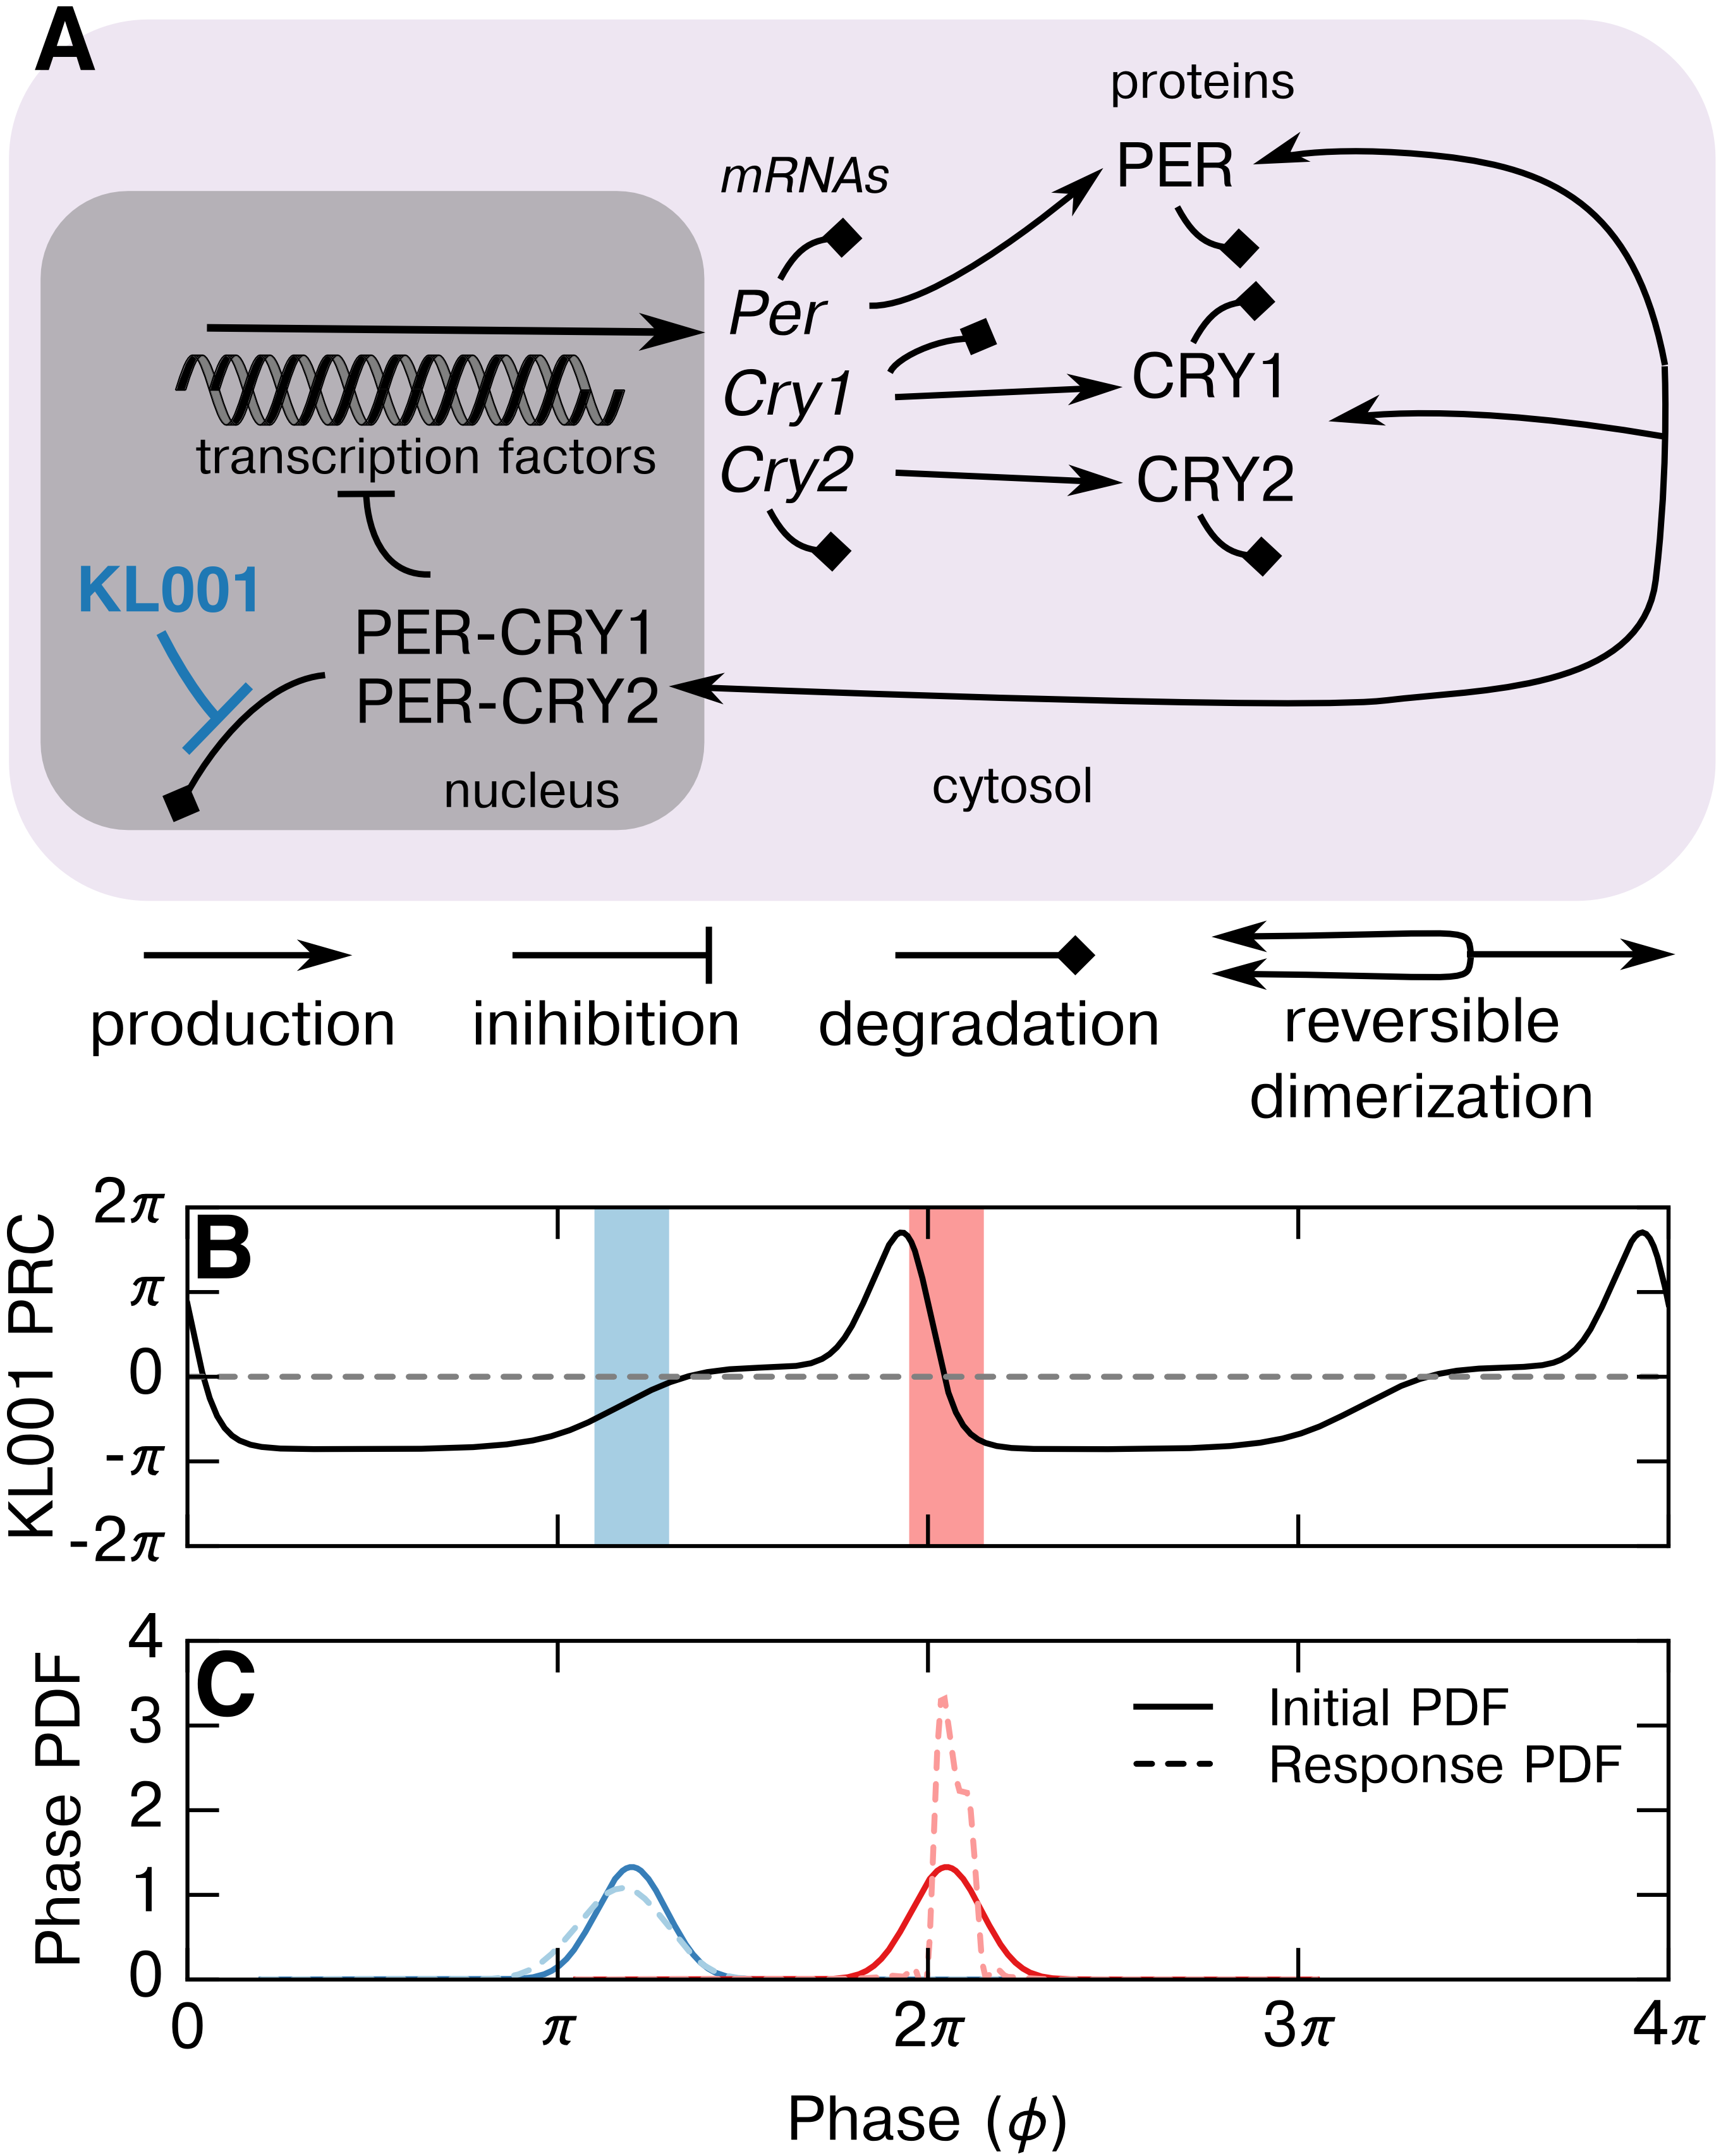
\includegraphics[width=7.5cm]{chap7/figures/fig1_diagram.png}
\end{center}
\caption{Schematic of mammalian circadian oscillator and effect of KL001. (\textbf{A}) Diagram of the core negative feedback loop driving mammalian circadian rhythms. This schematic is adapted from Figure \ref{fig:0} for easy reference. All states and reactions shown are included explicitly in the model (from \cite{StJohn2014a}) as shown in Table~\ref{tab:stjohnmodel}.
(\textbf{B}) Parametric infinitesimal PRC describing response to KL001 (reduction in parameter $v_{dCn}$). Note that this is double plotted to allow visualization.
(\textbf{C}) Synchrony of a population is affected by timing of KL001 application. Two example probability density functions (PDFs) of phase are plotted before (solid) and after (dashed) application of KL001 at the phases shown. In regions of positive slope (blue), the phase PDF is dispersed, whereas in regions of negative slope (red), the PDF is condensed, even though the mean phase is unchanged.}
\label{fig:fig1}
\end{figure}

\subsection*{Model reduction and the phase control problem}

Control of the circadian clock is primarily focused on shifting the phase of the circadian oscillator.
A unique phase $\phi \in[0,2\pi)$ may be assigned to each unique point on the limit cycle and as in the prior chapter, points in state-space that are not on the limit cycle may be assigned the phase of the point on the limit cycle to which they converge asymptotically in time. 
The 8-ODE oscillator may be reduced to a single ODE describing asymptotic phase ($\varphi$):
\begin{equation}\label{eq:cphase}
    \frac{d\varphi}{dt} = \omega + u(t)\cdot B(\varphi),
\end{equation}
where $\omega$ is the radial frequency ($2\pi/T$, where $T$ is period of oscillation), $u(t)$ is the control input, and $B(\varphi)$ is the infinitesimal parametric infinitesimal phase response curve (ipPRC) with respect to changing parameter $v_\text{dCn}$, as defined in the prior chapter and under the same assumptions.
This function may be calculated numerically in advance from the 8-ODE model by previously-defined methods \cite{Taylor2008,Abel2016b}.
The PRC is plotted in Fig.~\ref{fig:fig1}B.
One may consider the control input to be either ``speeding up'' or ``slowing down'' the oscillation depending on the sign of the PRC.
We opted to set the reference $\phi=0$ where the concentration of \textit{Per} mRNA is at a maximum.

As in the prior chapter, we are aiming to align the phase of the circadian oscillator ($\varphi$) with an external tracking phase (denoted $\varphi_r$), for example, the phase of the environment before and after a plane flight through multiple time zones or before and after beginning a shift work cycle.
This externally-imposed phase may be captured by a single ODE as well:
\begin{equation}\label{eq:ephase}
    \frac{d\varphi_r}{dt} = \omega +\Delta\phi\,\delta(t_{shift}),
\end{equation}
where $\Delta\phi \in [-\pi,\pi)$ is the phase shift of the environment that occurs at time $t_{shift}$, for example, when disembarking from the flight or starting a period of shift work.
We are searching for a control trajectory that will drive the oscillator $\varphi$ to external phase $\varphi_r$ and maintain it at $\varphi_r$ for all subsequent time. That is:
\begin{eqnarray*}
\lim_{t\to\infty} \|\varphi(t,u) - \varphi_r(t)\|&=&0.
\end{eqnarray*}


\subsection*{Control of single oscillator phase}
While light may be applied or removed instantaneously, pharmaceutical perturbation of the clock is constrained by pharmacokinetics.
To alleviate numerical complications arising due to unidentified (and likely nonlinear) pharmacokinetics, we selected a piecewise-constant parameterization of the control:
\begin{equation}
u(t) = u(t_k) \; \forall \; t_k \leq t < t_{k+1},
\end{equation}
and denote the sampling time $t_{k+1}-t_k$ as $\tau$.
For a predictive horizon of $N_p$ steps of duration $\tau$, we define
\begin{eqnarray}
U&\triangleq& \begin{bmatrix}
u(t_k) & u(t_k+\tau) & \cdots & u\left(t_k+(N_p-1)\tau\right)
\end{bmatrix}^\top
\end{eqnarray}
as the knots of the control trajectory defined at each of the $N_p$ steps.
To estimate the phase at the end of each step the phase dynamics in \eqref{eq:cphase} may be integrated over each of the $\ell \in \begin{bmatrix}1 & \cdots & N_p\end{bmatrix}$  steps to yield:
\begin{equation}\label{eq:discretephase}
    \hat\varphi(t_i+\ell\tau) = \varphi(t_i) + \frac{2\pi\ell\tau}{T}-\sum_{k=0}^{\ell-1} \int_{t_{k+i}}^{t_{k+1+i}} u(t_k)B(\varphi)\, dt,
\end{equation}
where $\hat \varphi$ is the predicted phase, $t_i$ is the current time, $\varphi(t_i)$ is measured, and the PRC is a function of $\hat{\varphi}$.
We define the phase error to be the magnitude of the phase difference between the predicted phase and the environmental phase:
\begin{subequations}
    \label{eq:phierror}
    \begin{eqnarray}
        e_\phi(\cdot) &\triangleq& \left|\angle\left(\exp(\mathrm{i}\hat\varphi(\cdot)-\mathrm{i}\varphi_r(\cdot))\right)\right|,
    \end{eqnarray}
    where $\mathrm{i}=\sqrt{-1}$. Computationally, driving phase error to $0$ is numerically unstable, so we relax the terminal constraint by ignoring phase error below a constant $\delta_\phi$:
    \begin{eqnarray}
    g_{\phi}(\cdot) & \triangleq &
        \begin{cases}
            0 & \text{if}\ e_\phi(\cdot)<\delta_\phi\\
            e_\phi(\cdot) & \text{otherwise}
        \end{cases}
    \end{eqnarray}
\end{subequations}
so that numerical imprecisions do not result in controller action.
Thus, the finite-horizon optimal control problem at each time $t_j$ may be solved for the optimal trajectory $u^\star$:
\begin{eqnarray}
        \nonumber \qquad u^\star &=& \arg\min_{U} \;\sum_{\ell=1}^{N_p} w^\phi_{\ell}g^2_{\phi}(t_i+\ell\tau) + w^u_{\ell-1}u^2(t_i+(\ell-1)\tau)\\
        \nonumber \text{subject to:}&&\\
        \label{eq:mpcoptim}   \hat\varphi(t_i+\ell\tau) &=& \varphi(t_i) + \frac{2\pi\ell\tau}{T}-\sum_{k=0}^{\ell-1} \int_{t_{k+i}}^{t_{k+1+i}}u(t_k)B(\varphi)\, dt,\\
     \nonumber  0 &\le& u_{\ell-1}\le \bar u, 
    \end{eqnarray}
for all $\ell=1, \cdots,N_p$, where $w^\phi_{\ell}$ and $w^u_{\ell-1}$ are positive weighting scalars evaluated at the end of the time step and start of the time step, respectively, as phase error is calculated after the control is applied for that step.
After identifying the optimal piecewise control trajectory $u^\star$, we applied $u^\star(t_i)$ to the full 8-state ODE model for $t \in (t_i, t_i+\tau]$ as is standard in model predictive control.

For this MPC formulation, $w^\phi$, $w^u$, $N_p$, and $\tau$ are design parameters which may vary.
We have selected:
\begin{align*}
w^\phi_{\ell} &= \ell,\\
w^u_{\ell-1} & = 1,
\end{align*}
for $ \ell=1,\cdots, N_p$.
We have elsewhere investigated optimal selection of design variables $N_p$ and $\tau$ for this exact formulation of MPC \cite{Abel2017a}. 
Based on these findings, we set $N_p=3$ (and $N_u=N_p$ where $N_u$ is the number of length of the control horizon) and $\tau=2$h, and instead studied the how phase control of a single oscillator differs from an oscillator population.




\subsection*{Case study \#1: nonlinear MPC for a single oscillator\label{ssec:applysc}}

To demonstrate the behavior of this controller, we applied it for the phase shifting control problem where a phase delay of 6h occurs at 12h (a phase delay of $\pi/4$ at a phase of $\pi$).
The environmental phase for this example was given by \ref{eq:ephase}, where $\Delta \phi=-\pi/2$, and $t_{shift} =12$h.
We used the Python language to solve the MPC problem, specifically, we used CasADi \cite{Andersson2012} and SciPy for formulation, and PySwarm to solve the nonlinear programming optimization problem.
Here, the numerical error in calculating phase was $\mathcal O(10^{-2})$ and so design variable $\delta_\phi = 0.1$.

The results of this simulation are shown in Fig.~\ref{fig:fig2}.
Briefly, the controller began its action at $t=12$h to achieve a phase delay.
The full $6$h phase delay could not be achieved within the initial negative region, and so the remainder of the shift was accomplished when the PRC returned to a negative value near 30h.
A decrease in amplitude occurred near $t=30$h due to transient deviation from the limit cycle, and the full amplitude returned for the following peak.

\begin{figure}[p]
    \begin{center}
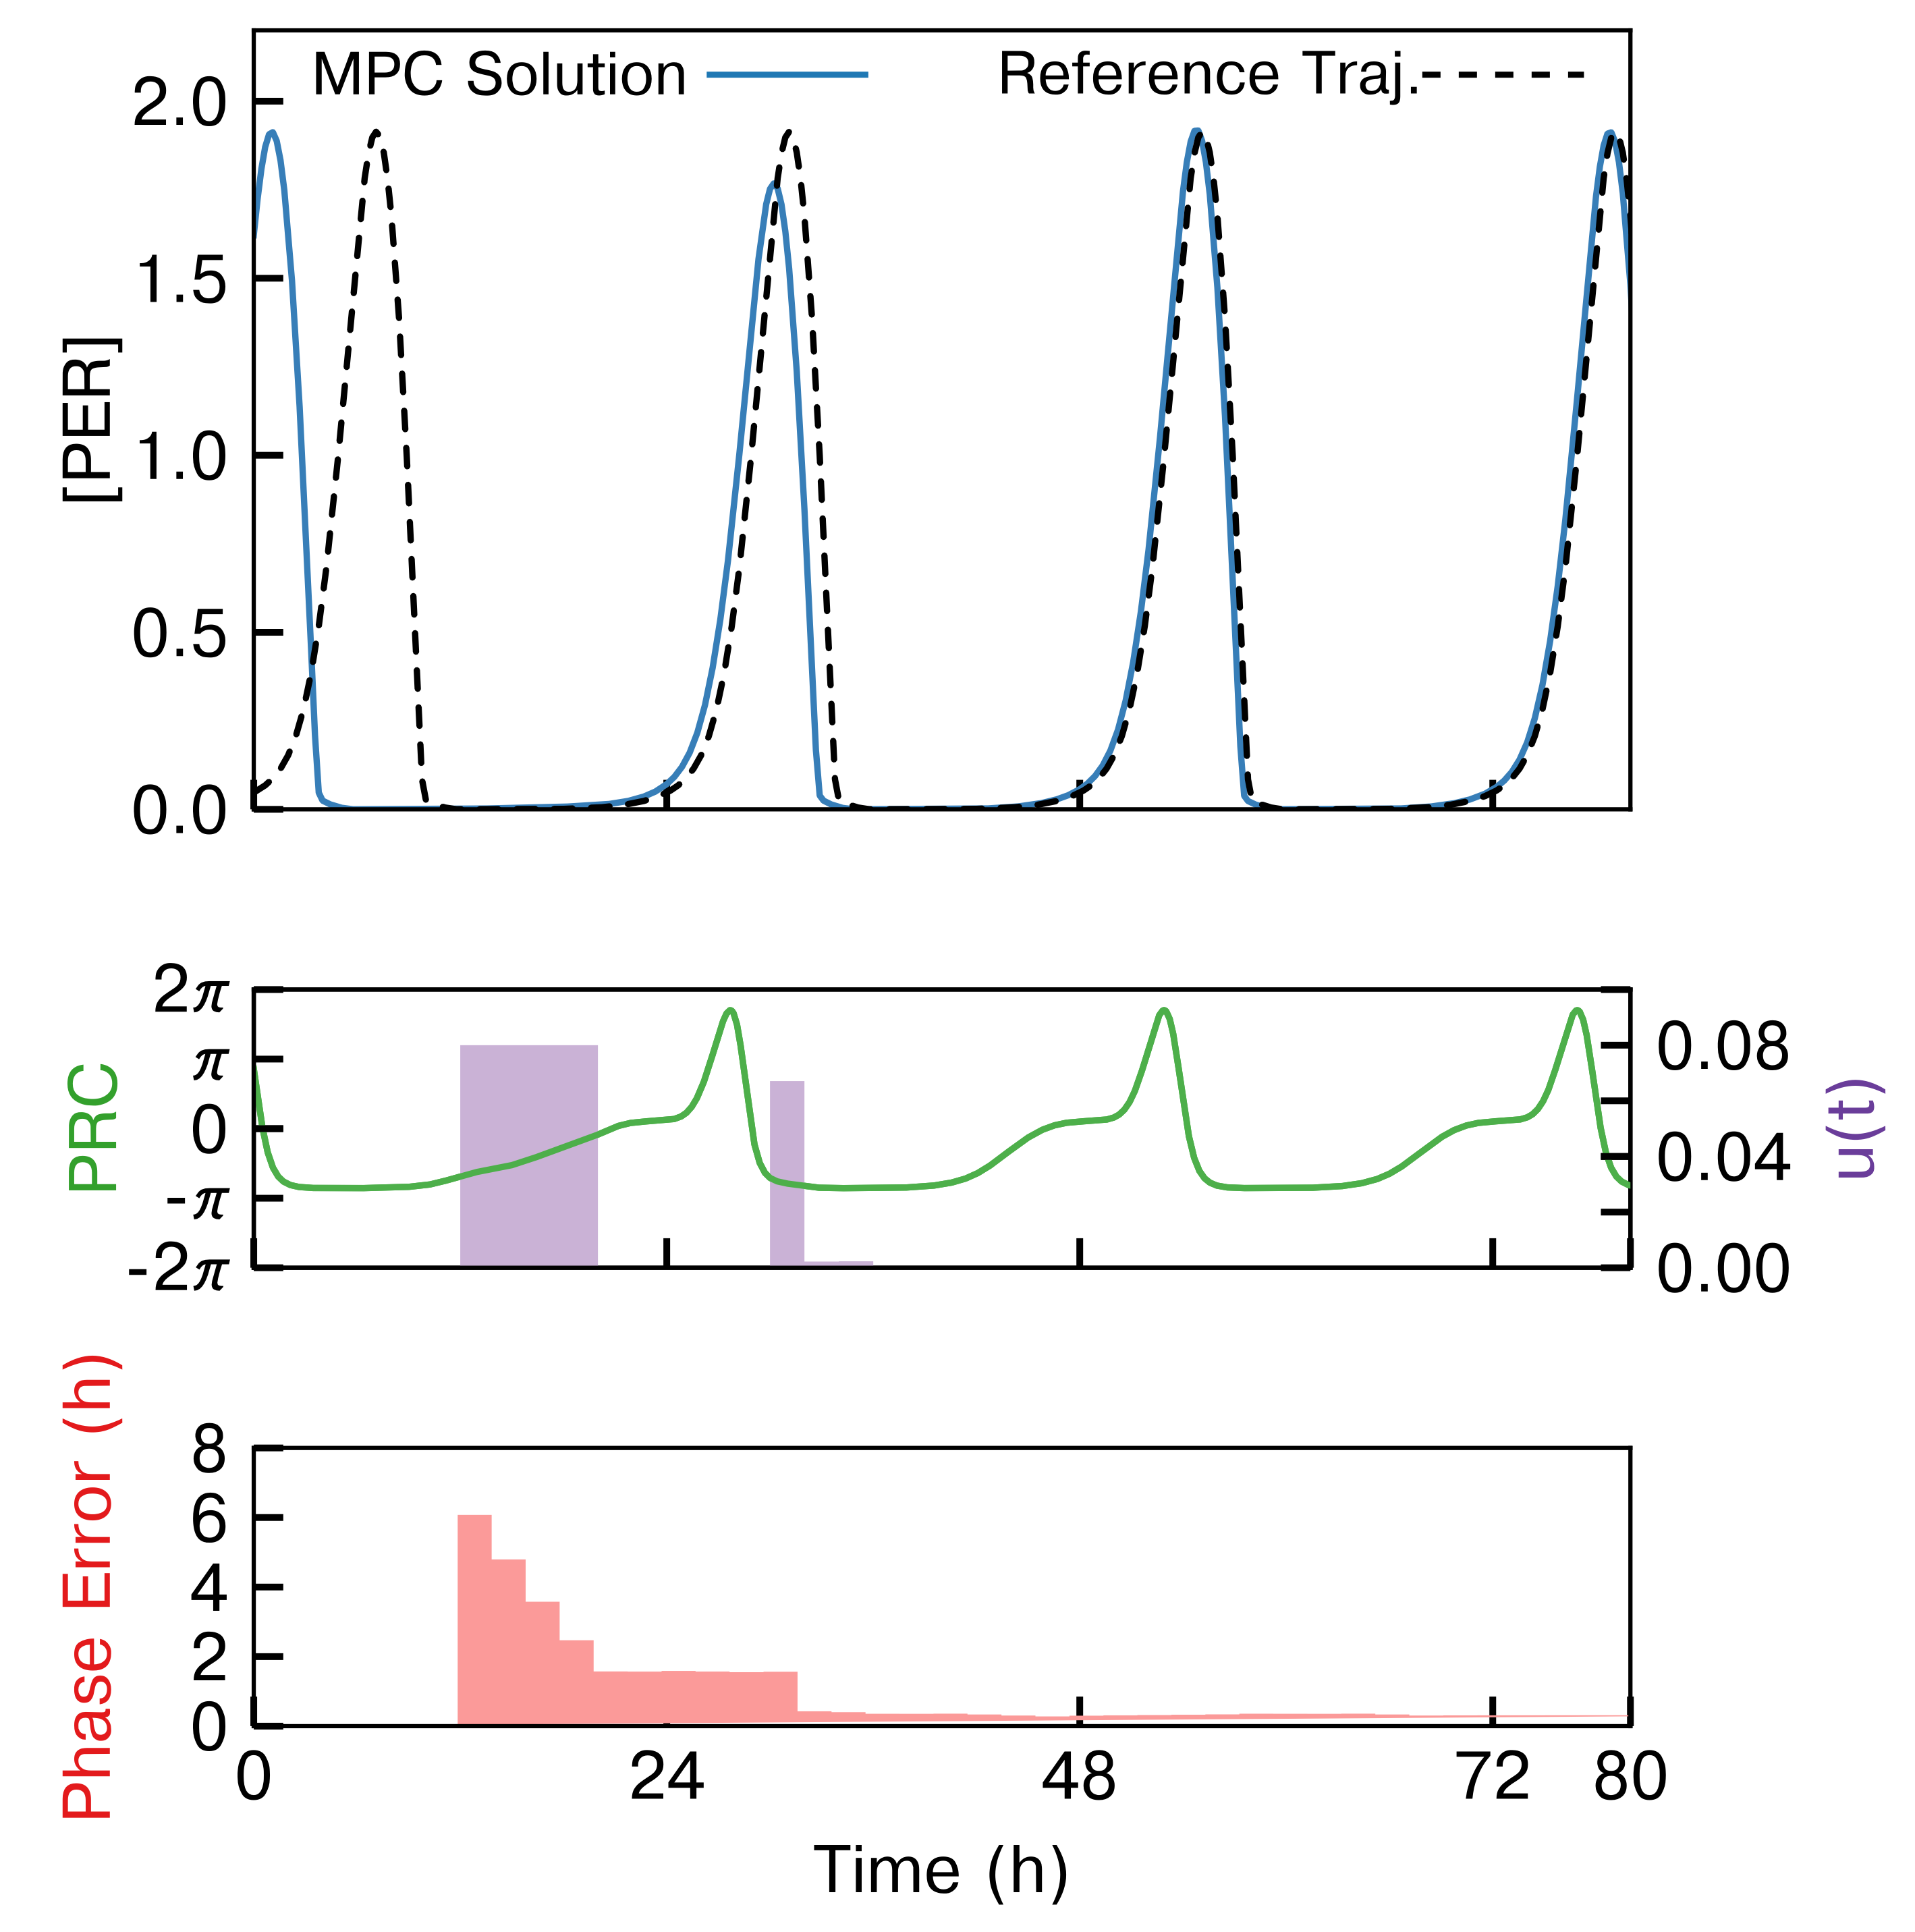
\includegraphics[width=7.5cm]{chap7/figures/fig2_single.png}
\end{center}
\caption{Application of the single-oscillator controller for a single oscillator achieving a phase delay of $6$h ($\Delta\phi = -\pi/2$) with $t_{shift} = 12$h. The controller acts immediately beginning at $t=12$h, and completes the phase delay to align with the desired reference trajectory after the PRC returns to a negative value. Note that the initial negative region of the PRC is elongated due to control slowing the advance of phase and maintaining the oscillator in a phase with a negative PRC for longer.}
\label{fig:fig2}       % Give a unique label
\end{figure}


\section{Control of population phase and synchrony}

The circadian oscillator is cell-autonomous, and each tissue is comprised of many thousands of individual oscillators.
While the SCN master pacemaker maintains its synchrony through intercellular communication, other tissues such as the liver lack paracrine signaling and are kept synchronized through a variety of identified and as-yet unidentified means, as guided by the SCN \cite{Welsh2010}.
The application of a pharmaceutical to any of these populations will affect this synchrony, and thus the amplitude of oscillation \cite{Ukai2007,StJohn2014b}.

While transient deviations from the limit-cycle eventually return to the limit-cycle amplitude, reduction in amplitude due to desynchrony will persist in the absence of signaling, making populations with weak coupling susceptible to long-term desynchrony from mistimed control.
The change in synchrony in response to perturbation may be calculated from the PRC \cite{StJohn2014b}.
In Fig.~\ref{fig:fig1}C we show how this may be intuitively understood based on the slope of the PRC: oscillator populations that lie on regions of positive slope result in the cells which are ahead in phase advancing further (or being delayed less) than oscillators which lag to begin with, broadening the probability density function (PDF) of phase.
Inversely, populations lying on a region of negative slope are condensed in phase by a similar argument.

Here, we first apply the previously-described controller to a population of uncoupled oscillators to demonstrate the deleterious effect of a population-agnostic nonlinear MPC on synchrony.
We then modify the MPC controller to explicitly penalize population desynchronization and demonstrate the ability to simultaneously control phase and synchrony of a population.

\subsection*{Case study \#2: limitation of single-oscillator assumption\label{ssec:scpop}}

We first applied the single-oscillator controller to a population of oscillators, with slight modification for tracking the mean phase of the population.
We modified the predictor in \eqref{eq:discretephase} to use the mean phase of the population $\bar{\varphi}$ rather than the phase of an individual oscillator:
\begin{equation}\label{eq:poppredictor}
    \hat\varphi(t_i+\ell\tau) = \bar{\varphi}(t_i) + \frac{2\pi\ell\tau}{\tau}-\sum_{k=0}^{\ell-1} \int_{t_{k+i}}^{t_{k+1+i}} u(t_k)B(\varphi)\, dt.
\end{equation}
Here, we calculated $\bar{\varphi}(t_i)$ from the phases of each oscillator $\varphi_n$ in the population by the parameter $z\in\mathbb C$ describing the population:
\begin{equation}
    z = \rho\,\exp(\mathrm{i}\bar{\varphi}) = \frac{1}{N}\sum_{n=1}^{N}\exp(\mathrm{i}\varphi_n),
\end{equation}
where $\rho$ is the Kuramoto order parameter, or colloquially, the synchrony index.
We emphasize that the controller did not observe any information about the population aside from its mean phase, and as such, the predictor \eqref{eq:discretephase} used in the finite horizon optimal control problem was imprecise due to slight differences between single-cell and population-mean phase response \cite{StJohn2014b}.
The controller was otherwise parameterized identically to that in the prior section.

Fig.~\ref{fig:fig3} shows the result of applying this controller to a population of 200 identical uncoupled oscillators with initial phases sampled from the PDF:
\begin{equation}\label{eq:wnbsol}
    p(\varphi) = f_{WN}(\varphi; \phi_0, \sigma),
\end{equation}
where $f_{WN}$ indicates a wrapped normal distribution with mean $\phi_0$ (set to $0$, to match the mean with the single oscillator case), and standard deviation $\sigma$ (set to $\pi/12$, approximately capturing the distribution of phases observed) \cite{StJohn2014b}.
As in the single-cell case, control was applied immediately starting at $t=12$h to begin correcting for the $6$h phase delay.
In the population case, this corresponds to a region of positive slope of the PRC, and intuitively resulted in a desynchronization of phase as evidenced by the decline in synchrony index for the duration of the KL001 pulse.
Despite the amplitudes of the individual oscillators (gray) returning after a transient to their pre-pulse levels, the population mean [PER] amplitude was reduced by approximately one-third due to desynchronization of the population.
Because there was no intercellular or external communication driving synchrony, the amplitude of the mean remained diminished for the duration of the simulation.

\begin{figure}[p]
    \begin{center}
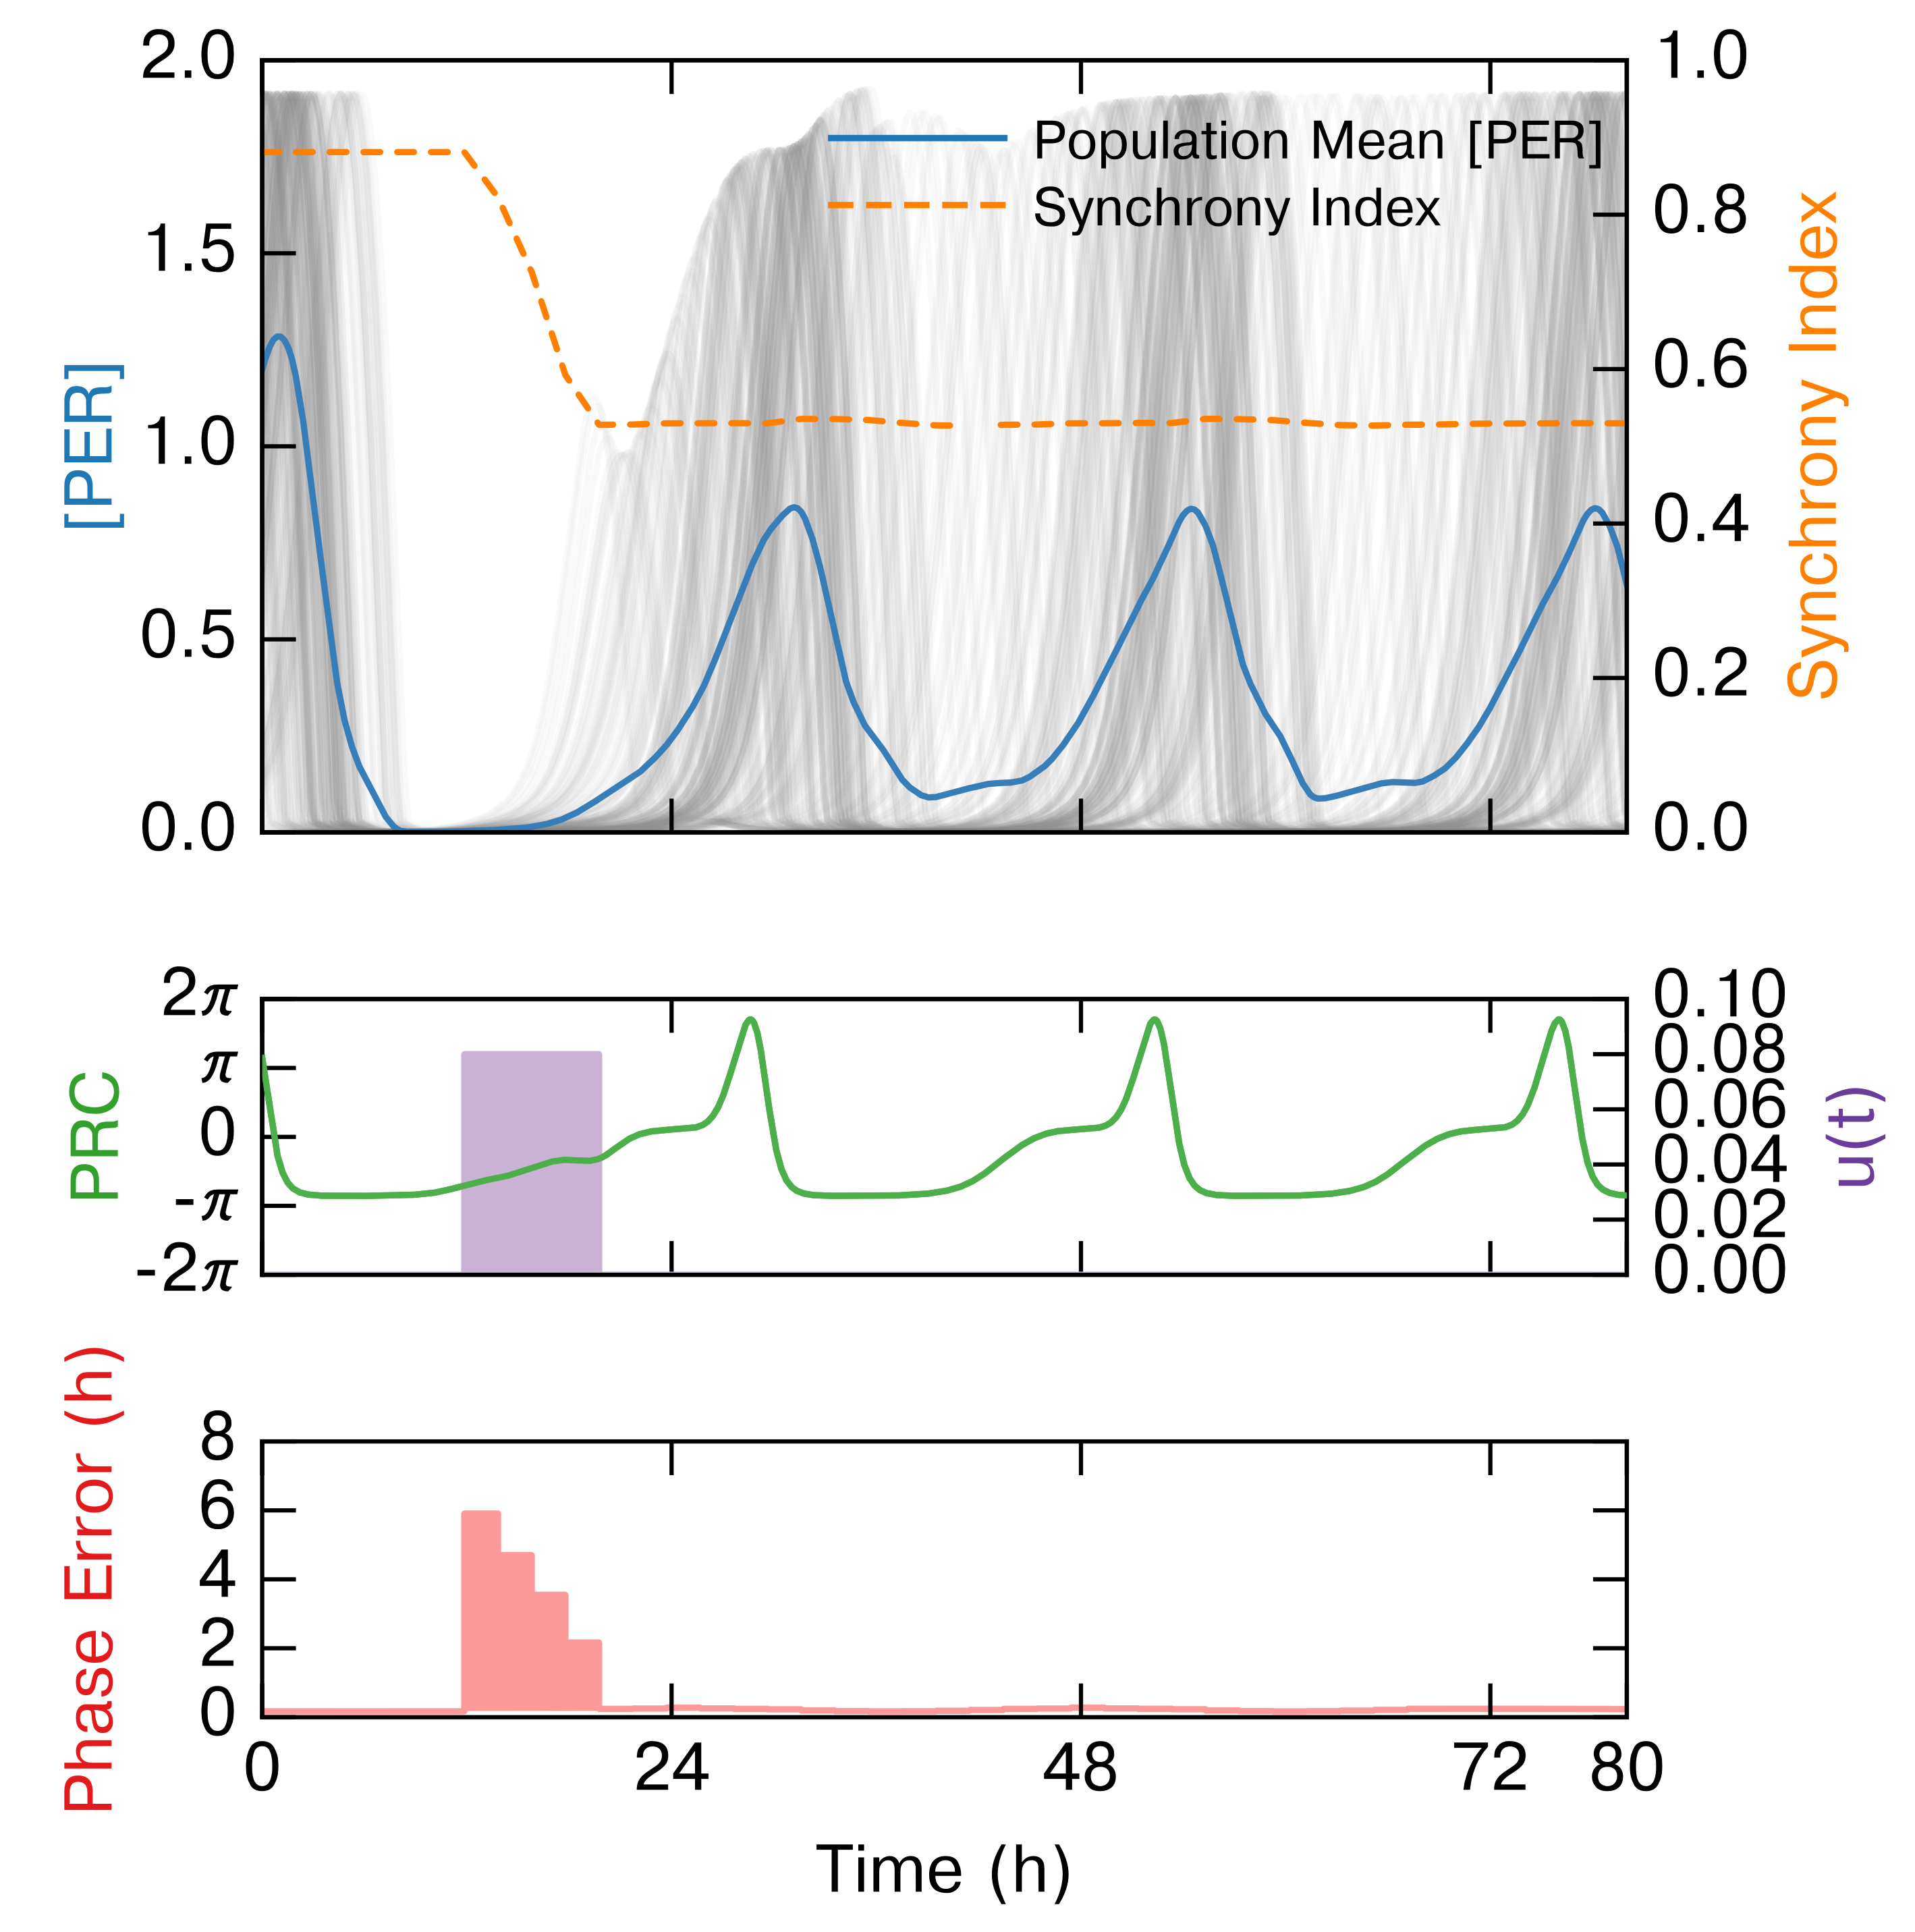
\includegraphics[width=7.5cm]{chap7/figures/fig3_population.png}
\end{center}
\caption{Application of the single-oscillator controller for a phase delay of $6$ h ($\Delta\phi = -\pi/2$) with $t_{shift} = 12$ h, for shifting mean phase of a population of 200 circadian oscillators (individual trajectories plotted in gray). While control is applied in nearly the same regions as Fig.~\ref{fig:fig1} and a $-6$ h shift was attained, this resulted in a dispersion of phase, a decrease in synchrony index, and a reduction in mean oscillatory amplitude.}
\label{fig:fig3}       % Give a unique label
\end{figure}

\subsection*{Population MPC algorithm for phase coherence \label{ssec:popmpc}}
A more sophisticated approach to control of an oscillator population involves predicting the evolution of the PDF itself rather than only mean phase.
Methods have been developed previously to compute the change in PDF directly in response to stimulation \cite{StJohn2014b}.
A change in variables allows the numerical computation of the new phase PDF:
\begin{equation}
    \hat p(\varphi, t)dh(\varphi) = p(\varphi, t)d\varphi,
\end{equation}
where $\hat p(\varphi, t)$ is the predicted PDF at time $t$ for phases $\varphi$, and $h(\varphi) = \varphi + \Delta\phi$, called the phase transition curve (PTC), is the total response to perturbation.
We may therefore revise the prediction model to explicitly involve calculation of the phase PDF at each step of the predictive horizon.
The PTC for each step within the predictive horizon may be calculated in a similar fashion to the predictor for the single-oscillator case:
\begin{equation}
    h_k(\varphi) = \varphi+ \frac{2\pi\tau}{T} -u(t_k) \int_{t_{k}}^{t_{k+1}}B(\varphi)\, dt,
\end{equation}
where $u$ is piecewise-constant and the integrand is a function of $\varphi$ which may be calculated numerically in advance as previously defined.
This function may be calculated numerically for each step, and used to calculate the evolution of the PDF:
\begin{equation}
    \hat p(\varphi, t_{k+1})dh_k(\varphi) = \hat p(\varphi, t_k)d\varphi.
\end{equation}
To calculate the first step, $\hat p(\varphi, t) = p(\varphi, t)$ is measured from the population under control.
The population predicted mean phase $\hat \varphi$ and synchrony index $\hat \rho$ may then be calculated from the predicted PDF:
\begin{equation}
    \hat\rho(t_k)\exp(\mathrm{i}\hat\varphi(t_k)) = \int_0^{2\pi} \hat p(\theta,t_k)\exp(\mathrm{i}\theta)d\theta,
\end{equation}
where $\theta$ is a dummy variable of phase. 
The phase error term $g_\phi$ may remain as defined in \eqref{eq:phierror}, and we define a similar error term penalizing desynchrony
   \begin{eqnarray}
    g_{\rho}(\cdot) & \triangleq &
        \begin{cases}
            0 & \text{if}\ \rho>\delta_\rho\\
            (1-\rho(\cdot)) & \text{otherwise}
        \end{cases}
    \end{eqnarray}
which reduces to 0 for a satisfactorily synchronized population.


Thus, the population control problem is:
\begin{eqnarray}
        \nonumber \qquad u^\star &=& \arg\min_{U} \;\mathcal J\\
        \nonumber \text{subject to:}&&\\       
        \nonumber \mathcal J &=& \sum_{\ell=1}^{N_p} w^\phi_{\ell}g^2_{\phi}(t_i+\ell\tau)+ w^\rho_{\ell}g^2_\rho(t_i+\ell\tau) + w^u_{\ell-1}u^2(t_i+(\ell-1)\tau),\\
        \nonumber  h_k(\varphi) &=& \frac{2\pi\tau}{T} -u(t_k) \int_{t_{k}}^{t_{k+1}}B(\varphi)\, dt,\\
        \label{eq:mpcPDFoptim} \hat p(\varphi, t_{k+1})dh_k(\varphi) &=& \hat p(\varphi, t_k)d\varphi\\
        \nonumber \hat\rho(t_k)\exp(\mathrm{i}\hat\varphi(t_k)) &=& \int_0^{2\pi} \hat p(\theta,t_k)\exp(\mathrm{i}\theta)d\theta\\
     \nonumber  0 &\le& u_{\ell-1}\le \bar u, 
\end{eqnarray}
where phase error and synchrony are calculated at the end of each step within the predictive horizon.





\subsection*{Case study \#3: implementation of population nonlinear MPC controller\label{ssec:popapply}}
As before, $w^{\phi}$, $w^u$, $w^\rho$, $N_p$ and $\tau$ are design parameters.
These parameters were set as before, with the exception of the new weighting of synchrony:
\begin{equation}
    \nonumber w^\rho = 10(\ell+1),
\end{equation}
which was set such that the synchrony term is of the same order of magnitude as the phase term, and increases to allow flexibility of synchrony early in the horizon.
Tuning this parameter will adjust the sensitivity of the controller to temporary desynchrony.
As $w^\rho \to \infty$, the controller will take no action unless it results in no loss of synchrony, i.e., the population lies completely on a region of negative slope of the PRC.
For lower but nonzero $w^\rho$, as in the case here, some flexibility is permitted, in that the controller may apply action that desynchronizes the population if it results in a large reduction in phase error.
Correspondingly, the controller will later resynchronize the population to account for this early desynchrony.
For $w^\rho=0$, the controller will behave as the popualtion-agnostic case.
After calculating the finite horizon optimal control $u^\star$, we apply the first step $u^\star(t_j)$ to all oscillators within the population for $t\in [t_j,t_j+\tau)$, and repeat this process.

    We applied the controller described in Sec.~\ref{ssec:popmpc} to the same phase shifting problem as the previous controllers: $t_{shift}=12$h, $\Delta\phi = -6$h.
The initial phase of the 200 uncoupled oscillators comprising the population was sampled from the PDF:
\begin{equation}
    p(\varphi) = f_{WN}(\varphi; \phi_0, \sigma),
\end{equation}
where $f_{WN}$ indicates a wrapped normal distribution with mean $\phi_0 = 0$ and standard deviation $\sigma=\pi/12$.

Results from this simulation are shown in Fig.~\ref{fig:fig4}.
The controller first applied input briefly in a slight desynchronizing region of the PRC, then paused for the remainder of the first negative PRC region due to the likelihood of further desynchronizing the population.
Once the population PDF returned to a region of negative PRC and a negative first derivative of the PRC the controller resumed input driving the population to its $6$h phase delay and restoring full synchrony.
Strikingly, changing the time of input resulted in a slight increase in the synchrony of the population in comparison to its original state, evidenced by an increase in the synchrony index.
Visually, this is evident from the clear alignment of individual oscillators within the population (plotted in gray) in comparison to the dispersion in phase evident in Fig.~\ref{fig:fig3} where synchrony was ignored.


\begin{figure}[p]
    \begin{center}
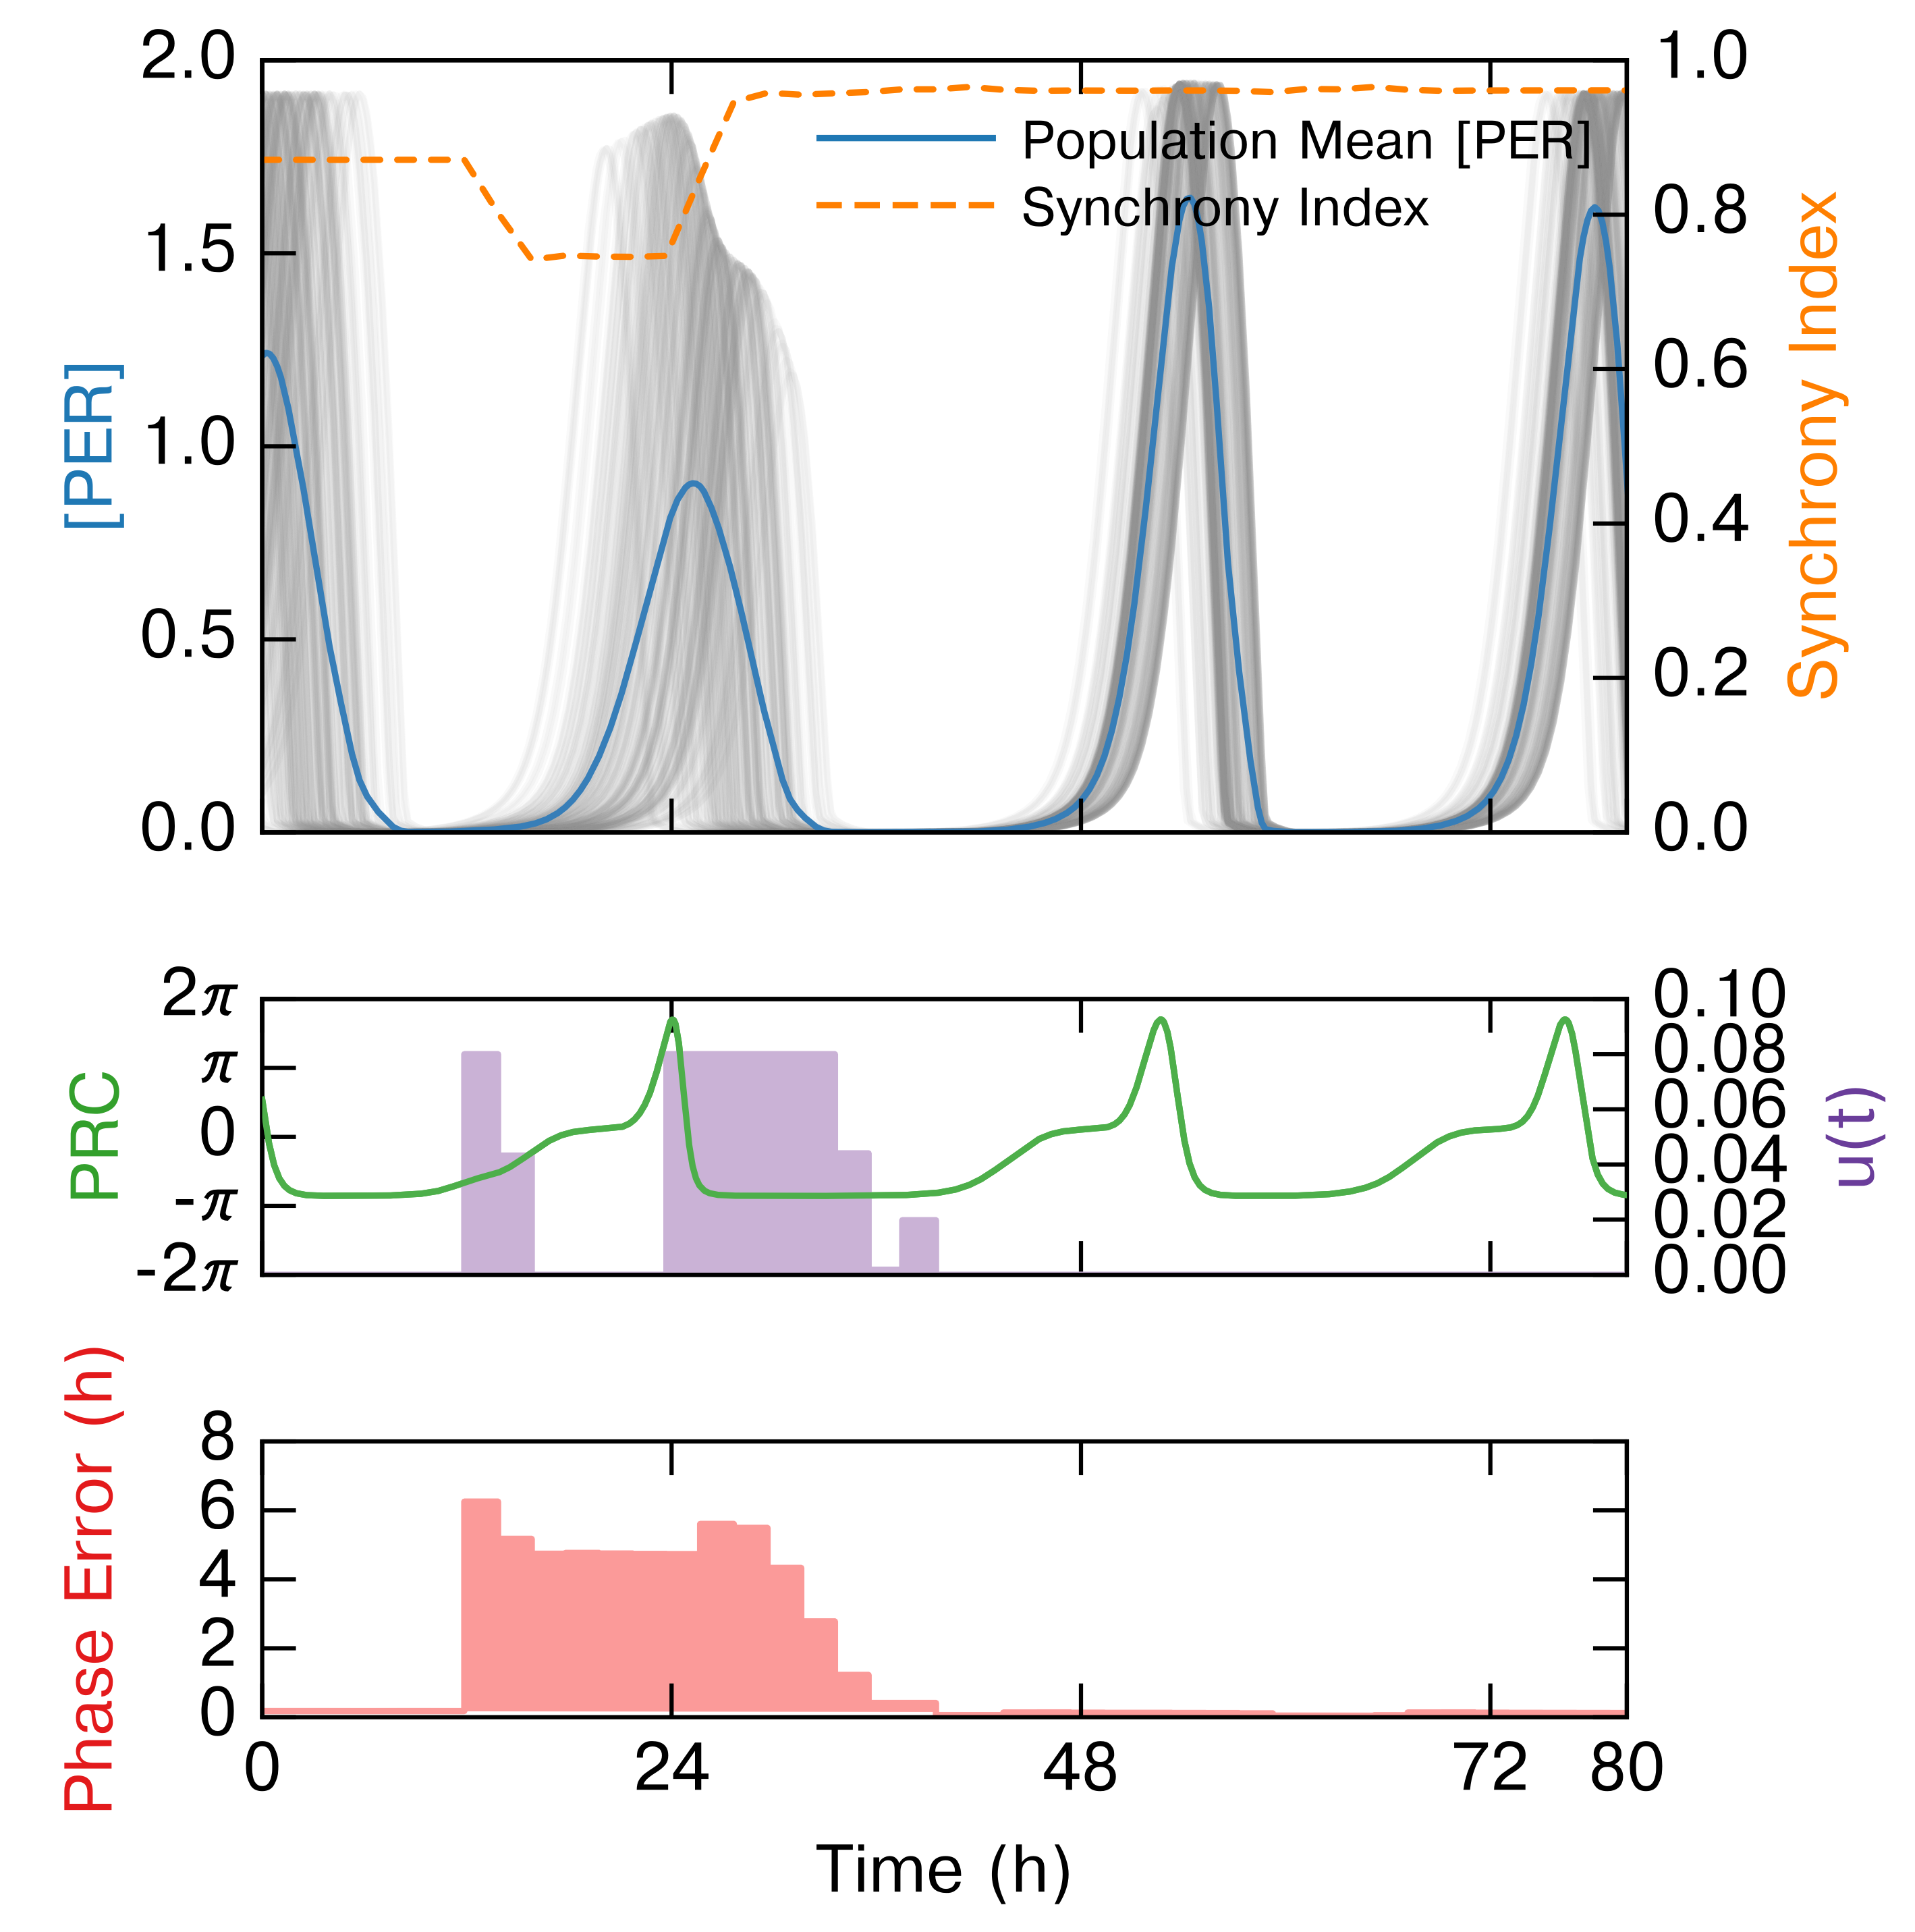
\includegraphics[width=7.5cm]{chap7/figures/fig4_population.png}
\end{center}
\caption{Application of the phase PDF controller to achieve a phase delay of $6$ h ($\Delta\phi = -\pi/2$) at $t_{shift} = 12$ h for a population of 200 oscillators (individual trajectories plotted in gray). This controller explicitly accounted for synchrony of the population. After a brief input to begin the shift, the controller delayed the majority of its input to find a region where population synchrony would be maintained. Indeed, synchrony is slightly improved by the control action, and a phase delay of $6h$ was achieved.}
\label{fig:fig4}       % Give a unique label
\end{figure}


\section{Summary\label{sec:conc}}
We have presented a modification of nonlinear MPC for phase manipulation of circadian oscillator populations, in which a PDF of phase is used in solving the finite horizon optimal control problem, allowing mean phase and population synchrony to be regulated simultaneously.
For many PRCs that have been calculated, there exists a region where the PRC or first derivative of the PRC is zero \cite{Dunlap2004}, it is therefore possible to manipulate phase and synchrony independently for a population of circadian oscillators through a single control input.
In reality, the ability to target these regions is limited by precision of the measurements of the PRC and population phase PDF.

One significant challenge in implementing this control algorithm \textit{in vitro} or \textit{in vivo} is the construction of an observer with sufficient accuracy to accurately reconstruct the phase PDF.
Current methods of assessing the phase of circadian oscillators relies on either noisy single-cell bioluminescent markers \textit{in vitro} or system level metrics \textit{in vivo} such as melatonin, activity, or body temperature.
However, even a simplistic assumption such as a wrapped normal PDF with an arbitrary estimate of standard deviation of phase could help avoid delivering control inputs where the slope of the PRC is expected to be positive, and thus help avoid desynchrony.
In this case, a long predictive horizon would quickly become inaccurate, however, necessitating careful selection of design variables $\tau$ and $N_p$.

Another challenge toward implementing such an algorithm is incorporating the as-yet uncharacterized pharmacokinetics and pharmacodynamics (PK/PD) for a small-molecule such as KL001.
This could potentially be achieved by including these terms directly in the prediction step of the MPC.
Uncertainty and individual variability in PK/PD measurements may reduce the accuracy of such an approach, however, further study is necessary to determine the extent of this variability, and how these inaccuracies affect controller performance.

It is our hope that these and similar control theoretic methods will inform the discovery of circadian therapies, and enable novel experimental design toward better understanding the dynamics of cellular populations and communication.














